This section demonstrates how to insert a float \ref{fig:subex} with subfigures \ref{fig:subex:pigs} and \ref{fig:subex:pig}.

\begin{figure}[!h]
  \centering
  \begin{subfigure}[b]{0.3\textwidth}
    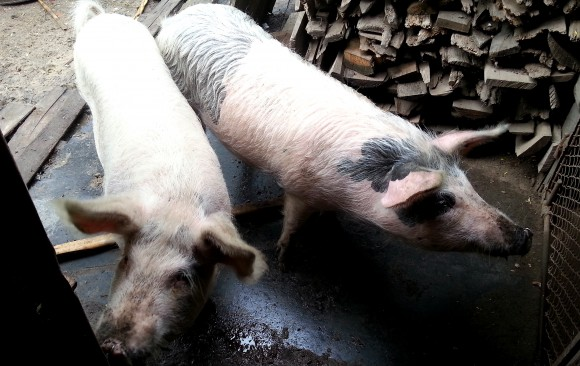
\includegraphics[width=\textwidth]{static/img/pigs1.jpg}
    \caption{Some pigs.}
    \label{fig:subex:pigs}
  \end{subfigure}
  \begin{subfigure}[b]{0.3\textwidth}
    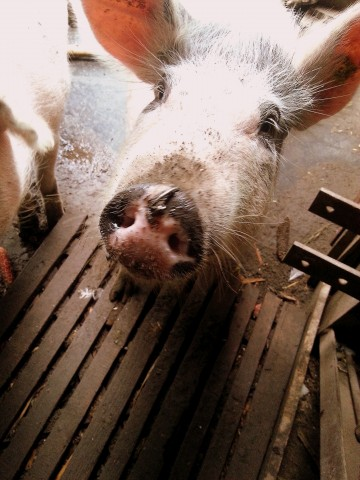
\includegraphics[width=\textwidth]{static/img/pigs2.jpg}
    \caption{A pig.}
    \label{fig:subex:pig}
  \end{subfigure}
  \caption{Some pigs being pigs.}
  \label{fig:subex}
\end{figure}